  \section{Предпосылки становления гомоморфного шифрования} \label{sec:ch1/sec1}

   Постараемся рассмотреть предпосылки становления такого современного научного направления, как гомоморфное шифроване. Прежде чем мы перейдем к рассмотрению соответствующей научной области, мы рассмотрим основные этапы развития теории информационной безопасности вообще. Обладая относительно недавней историей, гомоморфное шифрование является закономерным развитием как методов анализа, так и фундаментальной теории криптографии.\par
   Несмотря на то, что на сегодняшний день гомоморфное шифрование не поддается какой-либо строгой категоризации, для понимания процессов, которые вовлечены в это научное направление, важно предложить глубокий общий подход, который связан с динамикой развития фундаментальных исследований в других областях. Согласно этому подходу, можно условно выделить временные периоды  в теории криптографии и шифрования вообще, которые охватывают различные смежные дисциплины, как, например, теорию чисел или теорию вычислительной сложности.\par
   Постараемся выделить три таких периода, которые охватывают, условно говоря, различные временные масштабы, поэтому к ним больше применимо понятие „эры“.\par

   \subsection{Эра симметричного шифрования} \label{subsec:ch1/sec1/sub1}

    \color{Salmon}Во-первых, выделим эру симметричного шифрования, которая обусловила возможность существования гомоморфного шифрования в таком виде, в котором мы его видим сегодня. Она длилась приблизительно до 1970-х годов прошлого столетия, создав такие специфические понятия понятия, как блочный и потоковый шифр, ключ, открытый текст и т. д. \cite{KorobBasics-04}. Можно сказать, что эта эра изучает способы конфиденциального хранения информации. Секретный ключ, который позволяет сохранить конфиденциальность зашифрованной информации даже при компрометации всей системы шифрования, стал фундментальным понятием в криптографии и оказал наибольшее влияние на все последующее ее развитие \cite{NewDirs-76}.\par
    При этом сформировались также и определенные методы как шифрования так и анализа зашифрованного текста. Можно выделить такие классические методы шифрования, как замена, перестановка, гаммирование. Сам по себе теоретический аппарат в теории характеризуется медленным развитием, однако, в военные и послевоенные годы они получают мощный толчок, которому способствовали внешние условия: развитие радиосвязи, появление теории информации (Шеннон) и теории алгоритмов (Тьюринг). Теория информации обусловила появление способов изучения информационных свойств сообщений путем количественного анализа (так мы можем говорить, например, о переборе методом грубой силы), а теория алгоритмов обусловила практическое применение криптографии на вычислительных устройствах вместо механических, а также развитие теории вычислительной трудоемкости.\par
    Примером теоретических достижений в современной теории симметричного шифрования является появление концепции одноразового блокнота, появление таких алгоритмов для преобразования открытого текста в шифртекст, которые описываются не одиночными математическими операциями,  а сложными логическими примитивами, такими как, например, ячейки Фестеля, как следствие, появилась стандартизация  криптографических примитивов, и в дальнейшем блочных и потоковых шифров. Ярким образцом стандартизации является блочный шифр DES \cite{fips46-3}, представляющий собой набор документов и рекомендаций, утвержденных на государственном уровне и используемых в экспортной политике. \cite{SusanNewCentury-00}.\par
    Актуальным и одновременно отдельным направлением симметричного шифрования являются генераторы ПСП [Полуяненко-17], образующие криптографическую стойкость детерменированных устройств, операционных систем и многих криптографических пакетов,  таких, как OpenSSL. Для генераторов ПСП (или генераторов потокового шифрования)  наболее развитой областью является теория регистров сдвига с линейной обратной связью. Примерами являются генераторы Yarrow и LRNG. \cite{Yarrow-99}\cite{LRNG-18}\par
    Также можно выделить такое современное актуальное направление в симметричном, как аугментация существующих громоздких криптографических систем под нужны устройств с низкой вычислительной способностью, как, например, для интернета вещей. Это направление носит название легковесной криптографии, «Lightweight Cryptography». \cite{SoALightSymm-17}\par

   \subsection{Эра асимметричного шифрования} \label{subsec:ch1/sec1/sub2}

    \color{Blue}С 1970 годов можно обозначить начало эры ассиметричного шифрования, которая характеризуется фундаментально работой по RSA \cite{RSA-78}, реализовавшей обмен ключами Диффи-Хеллмана. Ассиметричные системы подняли новые вопросы не только для конфиденциального хранения информации, но также и для ее передачи, или, иначе говоря, они обусловили активное использование такого элемента, как канал связи в системах шифрования. Начинают формироваться методы анализа на основе комплексности/сложности проблем (NP-проблемы, P-проблемы и NP-полные), а также появляется понятие криптографических примитивов, например, односторонние функции. \cite{NewDirs-76}\par
    \color{ProcessBlue}Во второй эре можно выделить несколько этапов, длящихся, условно говоря, по одному десятилетию.\par

    \subsubsection{Первый этап эры асимметричного шифрования}

     Первый этап  1970-1980 гг. предлагает фундаментальные исследования и поиск новых математических примитивов благодаря работе \cite{NewDirs-76}, которая обозначила новое направление развития или другой угол зрения на тот момент в теории криптографии.\par
     Все это касается именно фундаментальной криптографии, здесь начинают формироваться сами категории криптографических примитивов и протоколов. Вводится понятие односторонней функции \cite{NewDirs-76}. Появляется многообразие протоколов, среди которых можно выделить разделение секрета \cite{ShamirShare-79} и электронную подпись \cite{DigSign-79}.\par
     Особое внимание получает теория чисел, благодаря которой \cite{NewDirs-76} создаются  предпосылки для изучения новых математических примитивов, например, конечных полей \cite{TakingRootsInFinite-77}, и вывислительных проблем, например, факторизации \cite{RSA-78}.\par
     Как уже говорилось выше, развитие получает теория вычислительной сложности \cite{ReduceNP-72}, вместе с которой появились другие модели атак по открытому тексту, шифртексту и выбранному шифртексту.\color{Red}Важной является теорема Брассарда о приведении к NP-полной задаче \cite{Brassard-79}.\par
     \color{Blue}Важно отметить также первую работу по гомоморфному шифрованию \cite{OnPrivData-78}, в которой оно определеляется под «приватным гомоморфизмом». Здесь эта область криптографии находится в состоянии зарождения, и более-менее интенсивное развитие гомоморфное шифрование получит лишь спустя несколько десятилетий.\par

    \subsubsection{Второй этап эры асимметричного шифрования}

     \color{Plum}Второй этап 1980-1990 гг. характеризуется дальнейшим развитием общей теории, но уже больше поисковыми и прикладными исследованиями, особенно в части новых криптографических протоколов. Все направления, зародившиеся на прошлом этапе также получают свое дальнейшее развитие.\par
     \color{Black}Изыскиваются новые вычислительные проблемы, которые обуславливают появление различных классов криптографических систем. Появляются вероятностные системы шифрования и вероятностный анализ. \color{Plum}Имевшая ранее более целостную структуру криптография подвергается пересмотру и более глубокому анализу, предлагая потенциальную возможность синтеза систем шифрования. Появляется понятие системы шифрования вообще, понятие системы с открытым ключом. Теория чисел и область, где она используется (простые числа, сравнения и модульная арифметика), даёт возможность строить такие системы на следующих вычислительных проблемах: факторизация, дискретный логарифм, квадратичный логарифм \cite{LOG-85}, возведение в степень \cite{RSA-78}. Появляется криптография на эллиптических кривых \cite{EllipticCurves-85}.\par
     Как уже было написано, продолжают исследоваться новые криптографические протоколы. Это направление проявляет себя, как наиболее активный процесс в исследованиях \cite[с.315/4]{NewDirsLater-97}. В результате появляются такие протоколы, как, например, протокол электронной подписи \cite{DigSign-79}, протокол забывчивой передачи \cite{ObliviousTransfer-88}, протокол сертифицированной почты \cite{ContractSign-85}, протоколы выборов \cite{ElectionScheme-85} \cite{SecretBallot-87} и др.\par
     Некоторые «фокусы» (невоспринимавшиеся всерьез умственные модели/абстакции) \cite{NewDirsLater-97}, например, с подбрасыванием монеты, начинают рассмативаться, как серьезная теория, которая становится основой в некоторых пртоколах, таких как, например, протоколы выборов и подбрасывания монеты \cite{BSecret-83} \cite{BCoin-82}. В дальнейшем это приводит к открытию теории доказательств с нулевым разглашением, сыгравшим большую роль в будущем контексте  вычислительной криптографии \cite{VerifySecretSharing-87} \cite{ComplexIntercativProofs-89}. Отметим также еще один шаг в направлении гомоморфного шифрования; он происходит совместно с работой по развитию приватного гомоморфизма \cite{OnPrivHomo-87}.\par
     \color{Cerulean}Наиболее важным событием, оказавшим большое влияние на фундаментальную теорию, можно исследование вероятностных систем шифрования \cite{ProbEnc-82}. Это позволило рассматривать криптосистемы с позиций набора новых  свойств, например, семантической защищённости, и новых примитивов: односторонних предикатов и функций с потайным входом. Это означает, что для потенциальной возможности синтеза криптосистем и, отдельно, систем шифрования, которая была описана выше, добавляются новые строительные блоки; появляется многообразие параметров, которые можно задавать и варьировать в процессе разработки системы.\par
     \color{Plum}В дальнейшем асимметричное шифрование находим множество практических применений, особенно, с развитием сети интернет.\par

    \subsubsection{Третий этап эры асимметричного шифрования}

     \normalcolor Третий этап 1990-2000 гг. – это этап усложнения и интеграции. В этом периоде исследователи обращают свой взор на выявление взаимосвязи в структуре теории вообще. Окончательно формируется теория анализа на основе комплексности. Кроме этого, исследователи обращают свое внимание на квантовую архитектуру, изучая методы анализа, применимые на ее основе. \cite{Foundatios-95}\par
     Интеграцию различных классов криптосистем друг в друга, а также их усложнение можно проследить, например, в разработке вероятностных доказательств с нулевым разглашением \cite{CSProofs-94}. Многие протоколы становятся многосторонними (multiparty computations) \cite{MultipartyGoldwasser-97}, и также формируется анализ, который принимает во внимание несколько сторон и возможности участников, например, атака Сивиллы. Здесь можно выделить «статические» (или классические) протоколы, например, протоколы торгов, выборов, совместной подписи и расшифрования или threshold-протоколы. Это протоколы, которые предлагает асимметричная криптография. Наряду с ним появляются «динамичные» (гомоморфные) протоколы, не имеющие прямое отношение к приватному гомоморфизму, но, тем не менее, развивающие его. Это протоколы анонимных запросов пользователей к базам данных (защищенные индексы) и совместные вычисления (запросы) баз данных между собой \cite{PrivateRetrival-97}. Развитие же самого приватного гомоморфизма можно обнаружить по косвенному влиянию. Авторы различных криптосистем сами пытаются исследовать свои системы на гомоморфные свойства. Все эти процессы происходят в рамках одной работы. Так, например, обнаруживается много систем с частичным гомоморфизмом \cite{OkamotoUchiyama-98} \cite{Paillier-99}. Появляются также примитивы, относящиеся непосредственно к вычислительной криптографии: позволяющие выделять определенные вычислительные механизмы из других систем NC-цепи \cite{NCComputing-99} и перешифрока шифртектса «на ходу» (Atomic Proxy Cryptography) \cite{AtomicProxy-98}.\par
     Усложнение прослеживается и в многообразии новых свойств, которые можно обнаружить теперь применительно к криптографической схеме, а не для шифртекста или его параметров. Такими свойствами являются, например, негибкость \cite{NonMalleable-99} \cite{MalleableCrypto-91}, семантическая защищенность \cite{ChoosenAnyOneWay-00}, «самоослепление» \cite{Paillier-99}, неразличимость, доверие, корректность, приватность, аутентификация, идентификация, анонимность, отслеживание, treshhold и т. д. Эти свойства получили определение, как придающие твердость \cite{Robustness, wiki} криптографической схеме. Как следствие для свойств твердости, обнаруживаются и новые  методы анализа, виды атак, например, приведение к другой (чаще полиноминальной) проблеме, компьютерная симуляция, случайная саморедукция \cite{SelfReduce-93}, случайный мэппинг. \cite[с.317/2]{NewDirsLater-97}\par
     За счет оказанного киптографией влияния окончательно формируется теоия комплексности, которая обнаруживает избыточность комбинаторных (ранцевых, knapsack) проблем \cite{Galore-93}.  С помощью теоремы Брассарда была сформулирована важная теорема о том, что детерменированная система или система с оператором эквивалентности обладает полиноминальной стойкостью и вскрывается за линейное время в отношении длины ключа \cite{BonehBlackBox-96}.\par
     К вниманию исследователей предстают новые вычислительные задачи, связанные с решетками и их применением \cite{WorstAverage-97} \cite{LatticesHard-96} \cite{CryptoLatticeReduction-97}. В итоге появляется криптография, которая основана решетках структур идеалов, например, колец, NTRU \cite{NTRU-98}. Работы предыдущих лет анализируются на предмет структуры и наличия проблемы решеток, к которым они при возможности, соответственно, сводятся. Кроме решеток, для всех остальных вычислительных задач, остаются изыскиваться только системы, построенные на проблемах факторизации (и другим проблемам теории чисел, которые связаны с конечным полем и понятием простого числа, например, задача о сумме подмножеств), линейным кодам и эллиптическим кривым.\par
     На примере AES можно выделить становление синтеза криптографических систем \cite{SusanNewCentury-00}. Несмотря на то, что в конкурсе участвовали кандидаты для блочных шифров, условия конкурса показывают, как можно задавать параметры для криптосистемы вообще. Можно также выделить направленность синтеза применительно именно к системам шифрования - грубо говоря, существует некоторый уровень абстракции, позволяющий строить системы шифрования различных классов по общим принципам.\par
     До сегодняшнего дня асимметричная криптография воспринимается, как наиболее используемое, комплексное и практичное направление, имеющее наиболее интенсивное развитие. Прослеживается тенденция развития и трансформации протоколов взаимодействия для двух сторон в многосторонние протоколы. Само понятие криптосистемы  прочно связалось с понятием асимметричной системы шифрования.\par
     Важно отметить, что асимметричная криптография не может отойти от концепции центральной базы данных, узлового источника, обладающего доверием. Именно на этой идее получает внимание вычислительная криптография, представленная следующей эрой.\par

   \subsection{Эра гомоморфного шифрования} \label{subsec:ch1/sec1/sub3}

    С 2000 гг. по настоящее время развивается эра гомоморфного шифрования. Ее можно охарактеризовать еще большими усложнениями, комплексностью, междисциплинарным взаимодействием, развитием технологии WWW. Вопросы криптографии, лежавшие на поверхности, теперь требуют более глубокого анализа, что повышает требования к квалификации исследователей. Формируется междисциплинарная связь между криптографией и другими научными областями, например, теорией множеств, теорией игр, теорией телекоммуникаций. \cite{DentCryptoCoding-03} Все это способствует условиям для обнаружения полностью гомоморфной системы шифрования. Эту также можно разделить на несколько периодов.\par

    \subsubsection{Первый этап эры гомоморфного шифрования}

     \color{Red}Первый этап 2000-2010 гг. является этапом междисциплинарной интеграции. Начинают захватываться области  различных компьютерных наук, как, распределенных вычисления, архитектура и пр. Так, например, появляются аппаратные криптографические акселераторы. \cite{Advances Crypto-07}. Появляется возможность стандартизации криптографических протоколов (IPSec и SSL).\par
     \color{LimeGreen}Усложнение и междисциплинарность можно продемонстрировать, например, в случае мультисторонних протоколов, которые приобретают элементы теории игр \cite{KatzGameTheory-08} \cite{HeindlMultivariate-09}. В 2000-х годах теория множеств оказывает влияние на криптографию, где ведется поиск новых математических структур, например, полукольца \cite{MonicoSemiRings-02} и якобианы \cite{GeneralizedJacobians-06}.\par
     Получает развитие теория решеток, а именно поблема худшего/среднего \cite{PeikertCollisionResistant-06} \cite{PeikertLatticesLog-07} \cite{MicciancioWorstCase-02} \cite{MultiBitLattice-07}. Как следствие, получает внимание и NTRU \cite{PhilipChoosingNTRU-09}\cite{NickHybridNTRUAttack-07}. В качестве новых вычислительных проблем, кроме решеток, можно выделить шифрование на основе 2-NDF формул \cite{2DNF-05}.\par
     Установился набор проблем, которые можно признать классическими в теории криптографии: для симметричного шифрования - логарифм, факторизация, возведение в степень \cite{RSA} \cite{ElGamal}, и, отдельно, ранцевая укладка \cite{LyubashevskyKnapsacks-06} \cite{MicciancioKnapsacks-07}; для ассиметричной криптографии -  модульная арифметика Диффи-Хеллмана, факторизация и логарифирования для систем RSA и Эль-Гамаля, цифровые подписи Шамира и, отдельно, ранцевая укладка Меркле \cite{HellmanOverview-02}. Для этих проблем, соответственно, появляются более глубокие методы анализа, например, адаптация алгоритма Полига-Хеллмана для редукции задачи дискретного логарифмирования \cite{MonicoSemiRings-02}.\par
     На фоне всего этого развиваются опасения, подкрепляемые теорией квантовых вычислений \cite{BarrenoQuantumFuture-02}.\par
     В конце-концов, исследователи постепенно приходят к системах неполного гомоморфного шифрования \cite{LatticeHomoVector-08} \cite{DamgardJurik-03} \cite{TOpMult-08} \cite{HomoNewApproach-08}. \color{Red}Развитие фундаментальных направлений, осознание взаимосвязей элементов криптографических систем позволило создать предпосылки для синтеза первой гомоморфной системы шифрования. \color{LimeGreen}Отдельно от этого развивается такое экзотическое направление, как вычисление ветвлений \cite{IshaiPaskinBranches-07}, которое можно поставить в один ряд с NC-цепями. Несмотря на то, что подобные работы лишь косвенно относятся к гомоморфному шифрованию, их все же можно приписать к более общей вычислительной криптографии. Но,  тем не менее, совокупность „косвенных“ работ внесет равнозначный вклад совместно с теорией решеток для работы Джентри \cite{Jentry-09}, которая исследует первую полностью гомоморфную систему шифрования в следующем этапе. \cite{DijkHomoIntegers-10}. К вычислительной криптографии относится и появление такой концепции, как обфускация данных. Это также говорит о стремлении  исследователей обеспечить приватность, но уже не данных, а самого кода или алгоритма для программы обработки. \cite{OnObfImpossible-01} \cite{IntervalObfuscation-09}\par

    \subsubsection{Второй этап эры гомоморфного шифрования}

     \color{Red}Наконец, 2010-2018 год – этап гомоморфного шифрования, облачных вычислений и, одновременно, период пост-квантовой криптографии; все направления можно признать равнозначными. \color{Green}Именно в последнее десятилетие системы гомоморфного шифрования получили наибольшее развитие \cite{AsurveyOnHomoEnc-16}. Вызвано это вниманием общества к, так называемым, облачным вычислениям. В виду некоторого появившегося разнообразия гомоморфных систем стала возможна их классификация.\par
     \color{Red}Выдвинутые в 1970-х годах Диффи и Хеллманом предположения о том, что NP-задачи устойчивы к атакам компьютерных алгоритмов, оказались неспособны противостоять системам на квантовой архитектуре. Представленный Шором 1994 году алгоритм позволяет с помощью свойства запоминания информации в кубитах эффективно распаралеливать NP-задачи. Кроме этого, прогресс в разработке квантовых компьютеров оказался достаточно быстрым, так что средняя организация уже к 2030 году сможет купить квантовый компьютер за 1kk долларов. Поэтому исследователи начинают обращать внимание на угрозы, исходящие от квантовых компьютеров. Алгоритмы, поддерживаемые NIST признаются слабыми; в них входят RSA, DSA и EC. Для оставшихся алгоритмов (AES) рекомендуемая длина ключа увеличивается  с 80 бит до 112 и 128 бит. \cite{NIST IR 8105}\par
     \color{PineGreen}Ведутся поиски новых примитивов, обладающих криптографической стойкостью для анализа алгоритмом Шора. В числе таких примитивов оказываются линейные коды, решетки и полиномы с множеством переменных (мультивариативные полиномы).\par
     Исследования Джентри, которое показало принципиальную возможность существования полностью гомоморфного шифрования, соответствующее направление «облачных вычислений» начинает занимать огромное влияние. Появляются улучшения для системы Джентри, исследуются новые полностью гомоморфные системы; также происходит процесс преобразования некоторых полностью гомоморфных системы в частично- и полностью гомомофрные системы с целью повышения производительно и более практических реализаций за счет ослабления гомоморфной структуры. Остаются открытыми некоторые вопросы безопасности гомоморфных систем, например, KDM, семантическая защищённость, устойчивость к атакам по выбранному шифртексту (устойчивость к атакам по подобранному шифртексту невозможна в-принципе, так как гомоморфный текст не негибкий). \cite{ASurveyOnHomoEnc-16}\par
     В качестве новых направлений для исследования в гомоморфном шифровании можно определить функциональное шифрование – это шифрование для выбранных атрибутов или для определенных пользователей, так назывемые системы шифрования с порогом (Threshold Full Homomorfic Encryption).\par
     Гомоморфное шифрование занимает свое место в теории криптографии, где криптография как бы пытается стать непрерывной, уйти от дискретных элементов.\par
     На данный момент разработаны эффективные алгоритмы полностью гомоморфного шифрования.\par

  \section{Теория гомоморфного шифрования} \label{sec:ch1/sec2}
   Работа Джентри позволила открыть существование полностью гомоморфных систем. Его результат - не просто конкретная схема, а набор инструментов и методик для получения таких схем, например, на основе ограниченно-гомоморфных систем. В-частности, это же может быть применимо и к гомоморфному шифрованию, как к основному элементу таких систем. Чтобы шифрование можно было назвать гомоморфным, оно должно позволять выполнение неограниченного числа операций над шифртекстом. Это подразумевает также, что должно выполняться следующее свойство - размер шифртекста должен оставаться в заданных пределах./par
   После схемы Джентри интерес к гомоморфному шифрованию значительно возрос во всем мире, наиболее значимые результаты были достигнуты в течении последних 10 лет.

   \color{Magenta}  
    Первой работой по гомоморфному шифрованию принято считать [RivestDataBanks-78]. Развитие описанные идеи получили в работе Брикеля и Якоби ``On privacy homomorphisms''. В течении последующих 30 лет удавалось получить лишь частичные результаты, то есть такие системы, где поддерживалось бы гомоморфное либо сложение, либо умножение, но ни обе операции вместе. Такие системы носят название, соответственно, частично гомоморфных систем (PHE). [AsurveyOnEncSchemes].

    В 1980-х со становлением вероятностной криптографии формируются требования к гомоморфным системам: способность выполнять любые операции (под любыми обычно понимаются умножение и сложение) в неограниченном количестве, обладать семантической защищенностью. Также должно выполнятся требование на ограниченное увеличение размера шифртекста после каждой операции, что косвенно отражает свойство отсутствия  ограничений на количество выполнений.

    Далее, в 1990-х теория алгоритмов позволила создать удобные представления для вычислений. Модель вычислений теперь может задаваться не только формулой, но и графом, таблицей истинности, булевой функцией, логической цепью, конечным автоматом и т. д. С 2000-х годов начинают развиваться почти гомоморфные системы  (Somewhat Homomorfic Encryption) -- это такие системы, которые могут выполнять как операции сложения, так и операции умножения, но в ограниченном количестве.

    Затем, начинают затрагиваться все уровни криптографической структуры, приводящее, таким образом, к тому, что Джентри синтезирует полностью гомоморфную систему, развитие которой вылилось в три поколения. В процессе развития этой системы, появилась возможность изучить особые свойства гомоморфных систем, появилась более глубокая теоретическая база. Кроме этого, появилось направление, которая уделяет особое внимание функциям вычислений -- обфускация. На данный момент гомоморфные криптосистемы имеют эффективные алгоритмы, а вектор их равития лежит в направлении интегрирования и дальнейшего усложнения.

    За все время была выработана следующая классификация для гомоморфного шифрования: частично-гомоморфное, ограниченно-гомоморфное и полностью гомоморфное шифрование.

\subsection{Частичное гомоморфное шифрование}

    Список частично-гомоморфных систем представлен ниже:
    \tiny
    \begin{longtable}{|p{0.1in}|p{0.3in}|p{0.7in}|p{0.2in}|p{0.2in}|p{0.9in}|p{0.7in}|p{1.3in}|}\hline 
        \#  & Год & Название & \multicolumn{2}{|p{0.4in}|}{Операции} & Вычислительная проблема & Улучшение какой системы & Примитив, свойства \\ \hline 
            & \multicolumn{7}{|p{4.3in}|}{Частично гомоморфные системы} \\ \hline 
        1   & 1978 & Система RSA &  & * & Факторизация [Montgomery-94] &  &  \\ \hline 
        2   & 1982 & Система Гольдвассер-Микали & ? &  & Проблема квадратичных вычетоа (Quadratic Residuosity Problem) [Kalinski-2005] &  & Вероятностная криптосистема, зашифровывает побитно \\ \hline 
        3   & 1985 & Система Эль-Гамаля &  & * & Дискретное логарифмирование [Kevin-90] & Система RSA &  \\ \hline 
        4   & 1994 & Система Бенало & + &  & Вычеты произвольной степени (Higher Residuosity Problem) [BenalohRooting-87] & Система Гольдвассер-Микали & Вероятностная криптосистема, зашифровывает блок данных в виде полинома \\ \hline 
            & 1998 & Система Накаша-Штерна & + &  & Вычеты произвольной степени (Higher Residuosity Problem) & Система Бенало & Улучшение производительности за счет изменения схемы расшифрования \\ \hline 
            & 1998 & Система Окамото-Утиямы & + &  & Квадратичные вычеты, факторизация & Система RSA, система Гольдвассер-Микали & Вероятностная криптосистема, улучшение производительности за счет использования других множеств \\ \hline 
        5   & 1999 & Система Пэйе & + & К & Комплексные вычеты (Сomposite Residuosity Problem) [Jager-12] &  & Можно добавить гомоморфное умножение, если знаешь открытый текст одного из сообщений, умножение на скаляр, вероятностная криптосистема \\ \hline 
            & 2001 & Система Дамгода-Джурика & + &  &  & Система Пэйе & Вероятностная криптосистема \\ \hline 
            & 2002 & Система Гэлбрейта & + &  &  & Система Пэйе & Эллиптические кривые \\ \hline 
            & 2007 & Система Кавачи & + &  & Поиск решения на решетках &  & Большая циклическая группа, решетки, псевдогомоморфизм \\ \hline 
    \end{longtable}
    \normalsize
\normalcolor
    Можно выделить следующие вычислительные проблемы, на которых может быть построен частичный гомоморфизм:

    \begin{enumerate}
        \item  Факторизация
        \item  Квадратичные вычеты, вычеты произвольной степени
        \item  Композитные вычеты
        \item  Решетки
        \item  Дискретное логарифмирования
        \item  Линейные коды
    \end{enumerate}
\normalcolor

\subsection{Ограниченно-гомоморфное шифрование}

\color{RoyalBlue}
    Отдельные механизмы были выработаны в классе ограниченно-гомоморфных систем. Особенностью этого класса является возможность конструирования функции, элементарные же функции состоят из базиса булевой алгебры.

    Для этого класса характерно использование бинарных таблиц и забывчивой передачи, как основных элементов при построении системы. Проблемы, которые необходимо решить при этом - это ограничение на рост размера шифртекста, а также реализация устойчивого протокола с фиксированным количеством раундов. В первой такой системе, которая припысывается Яо [Yao-82], участники общаются каждый раунд и узнают, нужна ли помощь в формировании выходного значения до тех пор, пока не будет пройдена вся цепочка вычислений. В этом случае глубина вычислений -- основной фактор, который влияет на комплексность криптосистемы.

    Система Сендера [Sender-99] является развитием системы Яо; в его системе в качестве входного значения используется полином, вычисляющийся с использованием NC-цепей, поэтому все операции происходят за один раунд. Однако, в этом случае размер шифртекста растет экспоненциально, так как основной ограничивающий фактор не глубина вычислений, а рамер бинарной таблицы. 

    Качественный скачок в развитии представляет система Бонеха-Го-Ниссима [Boneh-05], которая вычисляя 2-DNF-формулы над шифртекстом, обеспечивает как алгебраический набор операций, так и константный размер шифртекста.

    Система Ишая-Пашкина расширяет область гомоморфных вычислений на ациклические графы принятия решений, более генерализированным множеством, чем таблица истинности.

    Особенностью вышеперечисленных систем является использование бинарных операций вместо алгебраических, что не позволяет им полностью соответствовать классу алгебраически гомоморфных систем. Таким системы, также, являются особым случаем для теоремы Бонех и Липтона, которые показали, что детерминированные алгебраически гомоморфные системы над кольцами ${Z}/{NZ}$ могут быть сломаны за время не выражающееся экспоненциальной зависимостью. Но для систем ${Z}/{2}Z$ необходимо выполнение условия вероятностной системы, если они реализуют гомоморфные вычисления.

    \tiny
    \begin{longtable}{|p{0.1in}|p{0.3in}|p{0.6in}|p{0.2in}|p{0.3in}|p{0.7in}|p{0.8in}|p{1.3in}|} \hline 
    \#  & Год & Название & \multicolumn{2}{|p{0.5in}|}{Операции} & Математический примитив & Криптографический примитив & Размер шифртекста \\ \hline 
    1   & 1982 & Система Яо [Yao-82] & AND & OR & ${Z}/{2}Z$ & Искаженная схема (garbled circuit), забывчивая передача (oblivious transfer) & Растет линейно с каждой элементарной операцией; переменное количество раундов в протоколе, которая зависит от глубины вычислений \\ \hline 
    2   & 1994 & Система Феллоуза-Коблица, ``Polly Cracker'' & + & x &  &  & Размер шифртекста растет экспоненциально после каждой операции \\ \hline 
    3   & 1999 & Система Сендера [Sender-99] & AND & 1-OR\newline или\newline 1-NOT & ${Z}/{2}Z\left[x\right]$ & $NC^1$-цепи, забывчивая передача & Шифртекст растет экспоненциально, гомоморфизм на основе полугруппы, один раунд в протоколе \\ \hline 
    4   & 2005 & Система Бонеха-Го-Ниссима & + & 1-x & ${Z}/{2}Z\left[x\right]$ & 2-DNF формулы & Проблема подмножеств [Gjosteen-04], шифртекст имеет константный размер \\ \hline 
    5   & 2007 & Система Ишая-Пашкина & + &  &  & Ациклический граф (вычисление ветвлений, binary desicion diagrams) & Вероятностная криптосистема, не зависит от размера функции \\ \hline 
    \end{longtable}
    \normalsize
\normalcolor

    Отдельного внимания заслуживает система Мельчора [Melchor-10], которая опубликовалась после работы Джентри и которая разработала способ цепного шифрования, где каждое звено для этого шифрования может быть сформировано на основе примитива из другой существующей криптосистемы. Цепное шифрование позволяет производить гомоморфные вычисления заданной глубины, которая зависит от количества используемых примитивов их свойств, от чего также зависит наличие набора алгебраических операций.

\subsection{Полностью гомоморфное шифрованияе}

\color{Blue}
    Система Джентри в качестве своей основы использует решетки \cite{Jentry-09}, которые также получили огромное внимание после его работы. Решетки признаются устойчивыми к квантовому анализу \cite{Regev-06}, кроме этого они имеют достаточно обширный теоретический фундамент, поэтому их использование можно отнести к достоинствам системы. Теория решеток впервые была опубликована в \cite{Minkowski-68}, с тех пор было разработано несколько достаточно стойких вычислительных задач, наиболее используемыми из которых являются задачи поиска ближайшего  и кратчайшего вектора \cite{Peikert-15} и проблема среднего/худшего \cite{Atjai-96}. В \cite{Goldreich-97} выл представлен способ вычислительной редукции решеток, что напрямую связало их с теорией криптографии. Решетки могут комбинироваться с другими математическими примитивами, что определяет различные классы таких систем.\par

    \vspace{8mm}Так, например, система Джентри относится к классу систем, построенных на решетках идеалов. Подобное решение позволило реализовать ассиметриченую гомоморфную систему шифрования, то есть систему с публичным ключом \cite{Hoffstein-98}. Однако, она довольно сложна в реализации и имеет некоторые недостатки в плане производительности, особенно это касается перешифровки шифртекста. За последние годы было предложено много способов ее оптимизации. В 2010 году предложено улучшение схемы генерации ключа, а также улучшение стойкости гомоморфного шифрования \cite{Jentry-10}. Вариант схемы Джентри, работающий на шифртексте и ключе меньшего размера без потери стойкости был представлен в \cite{SmartVercauteren-10}. Поздние работы направлены на дальнешее улучшение алгоритма генерации ключа и также алгоритма "перешифровки" шифртекста. Также разработана ограничено-гомоморфная схема с пространством открытого текста большей мощности, что увеличивает количество гомоморфных операций \cite{Mikus-12}\par

   \vspace{8mm}Существует класс систем на решетках, которые используют проблему LWE \cite{Regev-09} и ее алгебраический вариант - ring-LWE \cite{Lyubashevsky-13}. Эти проблемы признаются наиболее стойкими, так как они позволяют использовать меньший размер шифртекста без потери защищенности. В 2011 году была предложена схема ограниченного гомоморфного шифрования \cite{BrakevskiVaikuntanathan-11} на основе RLWE, где была показана большая производительность, чем в LWE. Эта схема в той же работе была дополнена до полностью гомоморфной схемы.\par
    Все гомоморнфые схемы появившиеся после этой работы принадлежат к категории систем второго поколения, например, система использующая технику перелинеаризации \cite{BrakevskiVaikuntanathan-14}, которая устанавливает стабильный размер для шифртекста большого размера и обходится без процедуры перешифровки шифртекста. В качестве тенденций развития можно обозначить уровневые системы полностью гомоморфного шифрования, которые повышают производительность за счет использования функций с ограниченной глубиной вычислений (ограниченным набором элементарных операций) \cite{Brakerski-14}, линейный рост ошибки с каждой операцией \cite{Peikert-15}, а также системы с шифрованием атрибутов (идентификацией, множественными ключами) и собственными векторами \cite{Gentry-13}\par
    Актуальной схемой для доработки полностью гомоморфногом шифрования является схема \cite{Cheon-16}, которая использует проблему аппроксимации общего делителя, поддерживая большую мощность пространства сообщений.\par

    \vspace{8mm}\color{Orange}
    Одним из самых перспективных направлений в гомоморфном шифрованиии является класс NTRU-систем, также использующих решетки. В 2009 году NTRU упоминается в работе Джентри \cite[p.65]{Gentry-09}, как первая криптосистема, использующая структуры идеалов на решетках. Первая работа по NTRU  \cite{Hoffstein-98} была опубликована в 1988 году Хоффштейном, Пифером  и Сильверманом и изначально подразумевала собой криптосистему с публичным ключом на кольцах, которая лишь в дальнейших работах получила развитие и связь с решетками (1997-2001 год) \cite{Coppersmith-97,May-99,Gentry-01}. В дальнейшем NTRU-криптография строится вокруг работы Миклоша Айтая \cite{Ajtai-97}, на его принципе эквивалента среднего/худшего; цепочка работ, развивающих проблематику NTRU \cite{Micciancio-02,Peikert-06,,Peikert-07,Lyubashevsky-10,Micciancio-11} вышла в период с 2002 по 2007 годы. Параллельно работы Хоффштейна \cite{Hoffstein-98,Hoffstein-05} представили алгоритмы шифрования и электронной подписи, криптографическая стойкость которых была исследована в работе \cite{Stehlé-11}.\par
    Дальнейшее развитие NTRU получило с выходом серий работ, представляющих системы NTRU-LWE и NTRU Prime \cite{Bernstein-16}.\par
    Несмотря на то, что с момента появления NTRU-шифров прошло более двух десятилетий, NTRU-схема получила внимания лишь после открытия полностью гомоморфного шифрования и возросшего интереса к криптографии на решетках. Оба вопроса являются перспективными для NTRU, что делает его актуальным направлением в современной криптографии, особенно, учитывая что NTRU обладает хорошей асимптотической производительностью и малым размером шифртекста. \cite{Shor-99,HoffsteinLatticeCrypto-09}\par
\color{Blue}
    Возможность существования полностью гомоморфного шифрования на NTRU было впервые показано в \cite{Lopez-12} и \cite{Gentry-12}. Помимо проблемы решеток, система \cite{Lopez-12} также строится на мало изученной проблеме Decisional Small Polynomial Ratio (DSPR). В \cite{Bos-13} схема была избавлена от DSPR. Последовательно \cite{Brakerski-12} показал технику тензорирования, с помощью которой можно ограничить рост ошибки при гомоморфных операциях и также избавиться от DSRP. Однако, это техника требует большого размера ключа вычислений и комплексность в протоколе при ключевом переключении, что делает схему непрактичной. Все схемы, которые пытаются уйти от DSRP уязвимы к определенному виду атак. В 2016 году [Doroz-16] появилась модицифированная схема FHE для NTRU, не использующая DSRP и, кроме этого, не требующая ключ вычислений при произведении гомоморфных операций, что делает схему очень привлекательной для исследователей. Вместо этого она использует технику выравнимания шума \cite{Stehle-11}, которая была получена из схемы Джентри \cite{Jentry-13}.\par
    Актуальными направлениями для NTRU на данном этапе является дальнейшее получение практической FHE схемы, что является критически необходимым шагом, а также реализация вычислительного потенциала за счет оптимальной аппаратной реализации [Doroz-14,Dai-14,LiuWu-15]. Перспективной является также предложенная в 2014 году схема [Rohloff-14], где используются элементы самонастройки [Alperin-13] и "double-CRT" [Gentry-12] для преобразования шифртекстов в соответствии с текущей задачей.\par
\normalcolor


    \vspace{8mm}Одним из вариантов, не связанных с решетками, является схема, предложенная [VanDijk-10]. Эта схема использует ограниченно-гомоморфную схему, построенную на целых числах и модульной арифметике, которая затем использует метод Джентри для получения полностью гомоморфной схемы за счет "самонастройки" (bootstrapping).\par
Вычислительная сложность системы базируется на задаче аппроксимации поиска наибольшего общего делителя [Galbraith-16].\par
На данный момент реализована симметричная и ассиметричная гомоморфная система на целых числах; особенностью данной схемы является простота в реализации, взамен схема обладает низкой вычислительной способностью.\par
Основные направления развития данного класса систем включают уменьшение размера публичного ключа [Coron-11] [Coron-12] [Yang-12], а также улучшение алгоритмов генерации ключей [RamaiahKumari-12] и перешифровки [Chen-14]. Также существует версия с упаковкой шифртекстов [Cheon-13]\par
На данный момент существует множество подходов к улучшению системы на целых числах: масштбируемое инвариативное полностью гомомофное шифрование [Coron-14], схема с открытым текстом в виде целых чисел [RamaiahKumari-12], ограниченно-гомоморфная система с арифметикой больших чисел [Pisa-12], полностью гомоморфная схема без самонастройки [Aggarwal-14], а также схема в небинарном пространстве сообщений [NuidaKurosava-15].


\normalcolor


  \section{Криптографическая структура} \label{sec:ch1/sec3}
  
   \color{Melon}
    На основе анализа, произведенного выше, можно утверждать, что процесс развития криптографии последователен в направлении гомоморфного шифрования. Если симметричная криптография рассматривает вопросы конфиденциального хранения информации, то асимметричная криптография рассматривает вопросы конфиденциальной передачи информации, или, говоря по-другому, криптографические протоколы. Вычислительная криптография рассматривает аспект конфиденциальных вычислений, причем это относится как к данным, над которыми производятся вычисления, так и к алгоритму, по которому они производятся. Сама же последовательность развития заключается в том, что  симметричная криптография может быть интегрирована в асимметричную, а та в свою очередь может быть также интегрирована и рассмотрена с точки зрения вычислительной криптографии. Так, например, в криптографических системах асимметричный протокол исследуется для выработки и передачи секретных ключей, основной же канал передачи данных строится на основании симметичного шифра. В то же время как, и в симметричных, так и в ассиметричных системах могут быть обнаружены элементы гомоморфизма.\par
    Соответственно, не каждая система может обладать гомоморфными свойствами, и не каждый примитив из симметричной криптографии может использоваться при построении ассиметричной системы. Описанные отношения представлены на рисунке ниже.\par

    \begin{figure}[ht]
  \centering
  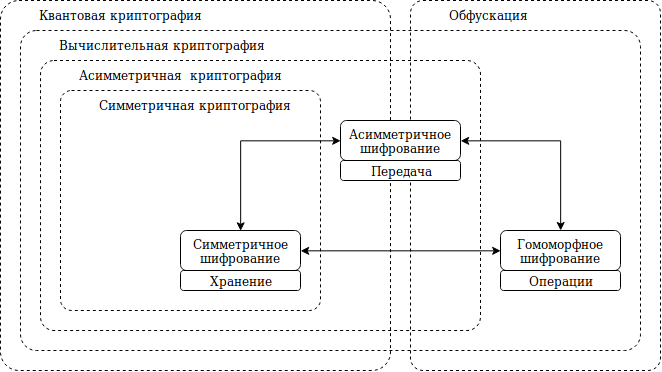
\includegraphics[scale=0.7]{share/struct.png}
  \caption{Криптографическая структура}
  \label{fig:struct}
\end{figure}


    \color{Goldenrod}Также на рисунке обозначены отдельно две области: квантовая криптография и обфускация. Обфускация сама по себе не является частью вычислительной криптографии, однако является производной от нее. В качестве довольно актуального направления, обфускация представляет собой способы обеспечения кофиденциальности, но не пользовательских данных, а самих алгоритмов обработки.\par
    Квантовая же криптография не затрагивает гомоморфное шифрование напрямую, но так как асимметричное или симметричное шифрование может быть частью системы с гомоморнфым шифрованием, то развитие этого направления может оказывать непосредственное влияние.\par
    \color{Plum}Чтобы показать динамику развития, можно отобразить условные элементы, которые представляют собой некоторый уровень абстракции над любой системой шифрования. Для этих элементов выделяются четыре уровня абстракции. Эти уровни затрагиваются в различной мере на различных этапах развития теории шифрования и криптографии, за счет чего и обладают качеством выражения динамических свойств. Этими уровнями являются:  уровень вычислительной проблемы, уровень математических примитивов, уровень криптографических примитивов и уровень криптографической схемы.\par

    \begin{figure}[ht]
  \centering
  
\includegraphics[scale=0.7]{share/el.png}
  \caption{элементы системы гомоморфного шифрования}
  \label{fig:struct}
\end{figure}


    \color{ProcessBlue}Вычислительная проблема характеризует, насколько величина перебора входных данных по значению шифртекста близка по сравнению с граничным значением, представляющим экспоненциальную зависимость от длины шифртекста (значение 2 в степени длины шифртекста). Иными словами, она характеризует качество того, что входные данные нельзя подобрать за время, имеющее полиноминальную зависимость от длины шифртекста.\par
    Набор математических примитивов задаёт множество значений (символов) для шифртекста, его структуру, а также определяет элементарные операции над ним, которые образуют уровень вычислительной проблемы - параметр, связывающий преобразования из открытого текста в шифртекст.\par
    То, какую задачу организует вычислительная проблема посредством математических примтивов, а также функциональное назначение криптосистемы в целом задают криптографические примитивы, например, односторонние функции. Криптографический примитив в системе шифрования определяет, как вычислительная проблема может быть редуцирована, то есть обеспечивает существование неких секретов или ключей.\par
    Наконец, криптографическая схема реализует непосредственно понятие ключа и протокола, то есть модель для конечного использования всей криптосистемы (системы шифрования).\par
    Можно увидеть, что на заре развития теории криптографии, основополагающими уровнем был уровень криптографического примитива, на основе которого изыскивались различные методы шифрования. До асимметричной криптографии никто не мог предположить наличие элементов для криптографической схемы, поэтому можно сказать, что уровни криптографических примитивов и криптографической схемы совпадают, то есть для эры симметричного шифрования не было четкого разделения на уровне вообще, как и понятия системы шифрования.\par
    C появлением асимметричной криптографии появилось наличие публичного/секретного ключа, которым описывается работа криптографической схемы.\color{RoyalBlue}Для этой эры характерно четкое осознание всех уровней, но основные направления исследований сосредоточены на области информационных процессов и протоколов, в которую входят криптографические примитивы и криптографическая схема.\par
    В конце второй эры и начале третьей, внимание ученых сосредоточено на фундаментальных проблемах и, соответственно, на математической области. Можно утверждать в полной мере, что сейчас ученые могут определять и вычислительную область, которая по своей сути обращается на взаимодействие между математическими и криптографическими примитивами. В этом случае, математическая область составляется как бы мощность гомоморфных вычислений, ту ошибку, которая накапливается после каждой операции, а область информационных процессов составляет некий количественный буфер, способность выдерживать эту ошибку. Гомоморфное шифрование имеет непосредсвенную зависимость от математических и криптографических примитивов, отражая таким образом как межуровневую связь, так и связь с различными областями.\par
\normalcolor


  \section{Итоги} \label{sec:ch1/sec4}
   
       Подведём итоги развития гомоморфного шифрования и выделим актуальные направления развития.
    \begin{enumerate}
        \item Вычислительные проблемы
		\begin{enumerate}
			\item Модульная арифметика
		            \begin{enumerate}
                              \item Факторизация
                              \item Квадратичные вычеты
                              \item Композитные вычеты
                              \item Вычеты произвольной степени
                              \item Дискретное логарифмирование
                              \item Поиск наибольшего делителя
                        \end{enumerate}
			\item Решетки
		            \begin{enumerate}
			            \item Проблема проблема эквивалента среднего/худшего базиса
			            \item Прооблема кратчайшего вектора
			            \item Аппроксимация среднего вектора
                              \item Проблема соседнего вектора
                        \end{enumerate}
			\item Обучение с ошибками
		            \begin{enumerate}
			            \item Обучение с ошибками в пространстве колец
                        \end{enumerate}
			\item Комбинаторные проблемы
		            \begin{enumerate}
                              \item Укладка рюкзака
			            \item Subset-sum
                              \item Раскраска графа
                        \end{enumerate}
		\end{enumerate}
	\item Математические примитивы
		\begin{enumerate}
			\item Бинарная логика
			\item Пространство остатков целых чисел 
			\item Идеалы
			\item Усеченые кольца
			\item Линейные коды
                  \item Биллинейные спаривания на эллиптических кривых
		\end{enumerate}
        \item Криптографические примитивы
		\begin{enumerate}      
                  \item Atomic proxy cryptography
		      \begin{enumerate}
                        \item Самонастройка (bootstraping)
			      \item Перешифровка (refleshing)
			      \item Упаковка шифртекста
			      \item Пороговое ограничение шифртекста (перелинеаризация)
		      \end{enumerate}
                  \item Односторонняя функция
                  \item Забывчивая передача
                  \item Защищенные индексы
		\end{enumerate}
	\item Криптографические схемы
		\begin{enumerate}
	            \item Вычисление функций
		            \begin{enumerate}
	                        \item Искаженная схема
	                        \item $NC^{1}$-цепи
                              \item Формулы 2-DNF
                              \item Ациклические графы
		            \end{enumerate}
	            \item Пороговое шифрование
		            \begin{enumerate}
	                        \item Шифрование атрибутов
	                        \item Выборочная идентификация
		            \end{enumerate}
	            \item Гомоморфность
		            \begin{enumerate}
	                        \item Частичная
	                        \item Ограниченная
                              \item Полная
		            \end{enumerate}
	            \item Обфускация
	            \item Арифметика больших чисел
	            \item Публичный ключ
		\end{enumerate}
    \end{enumerate}




